
\noindent
Integrating curvilinear geometries into modeling software is an involved multi-level process. It requires meshing software capable of creating accurate higher order elements from analytic designs or experimental data, a curvilinear grid manager able to efficiently manipulate such elements, as well as a PDE solver able to benefit from the curved geometries. The latter is mainly achieved by means of curvilinear basis functions able to accurately describe the associated vector fields (e.g. \textit{div} or \textit{curl}-conforming), adapting to the non-linear "bending of space". Ideas of using curvilinear grids first appeared in the literature in the 1970s \citep{ciarlet+1972, lenoir1986} and have been used in electromagnetic simulations for at least two decades \citep{wang+1993}. \\

%%
\noindent
An impressive example of using a curvilinear $3$-dimensional code together with DG and optimized for parallel GPU processing can be found in the aerodynamics community \cite{Warburton2012}.
%%
Wang et. al. \cite{wang+2011} demonstrate a 3D curvilinear parallel DGTD (\textit{Time-Domain}) code for solving Maxwell's equations in a homogeneous medium.
%%
Nevertheless, in electromagnetic community curvilinear grids are much less widespread than linear, predominantly used in 2D codes \citep{wang+2011a}.
%%
We believe that the associated challenges are as follows
\begin{itemize}
\item The generation of curvilinear meshes is a challenging process, as naive approaches can result in self-intersecting meshes \citep{toulorge+2013, johnen+2012}. Further, it must be ensured that the generated elements are optimal for the optimal PDE convergence \cite{lenoir1986}.
\item Standard functionality of a grid manager, such as interpolation, local-to-global and global-to-local mappings, integration, calculation of normals and basis functions becomes significantly more difficult in the curvilinear case; additional numerical tools, such as \textit{Lagrange} interpolation, adaptive integration, symbolic polynomial manipulation, and optimization algorithms are needed to provide the desired functionality. 
\item In order to fully benefit from the curvilinear geometries through reducing the total element count, basis functions of order sufficient to resolve the detailed structure of the field are necessary. The widely used CG-based codes require a divergenceless curvilinear basis of flexible order that preserves the field continuity across the element boundary. At the moment of writing authors are not aware of publications presenting such a basis. Fahs\cite{fahs2011} implements a serial 2D and 3D curvilinear DGTD code using polynomially-complete basis, and studies the scaling of the accuracy of electromagnetic benchmarks (\textit{Mie} scattering and layered \textit{Mie} scattering) depending on $p$-refinement. He finds that only in curvilinear geometries increasing the basis function order significantly improves the solution accuracy.
\end{itemize}

\noindent
Until recently, literature presents implementations of curvilinear electromagnetic DGFD codes with several simplifications, limiting the flexibility and detail achievable with moderate computational resources. \\

\noindent
The major objective for PDE solver optimization is the improvement of accuracy of the PDE solution given a limited computational resource, and curvilinear geometries can offer that. The curvilinear material boundaries decrease or fully eliminate the artificially high jump in the surface derivatives \cref{fig:result:spherecurv}, avoiding the unphysical "corner effects" \cite{volakis1998, jin2014}. Otherwise, the corners have to be smoothened by high \textit{h}-refinement, which leads to unnecessarily high number of \textit{Degrees of Freedom} (DoF). \\

\begin{figure}
    \centering
	\begin{subfigure}[b]{0.48\textwidth} \hspace{8mm} 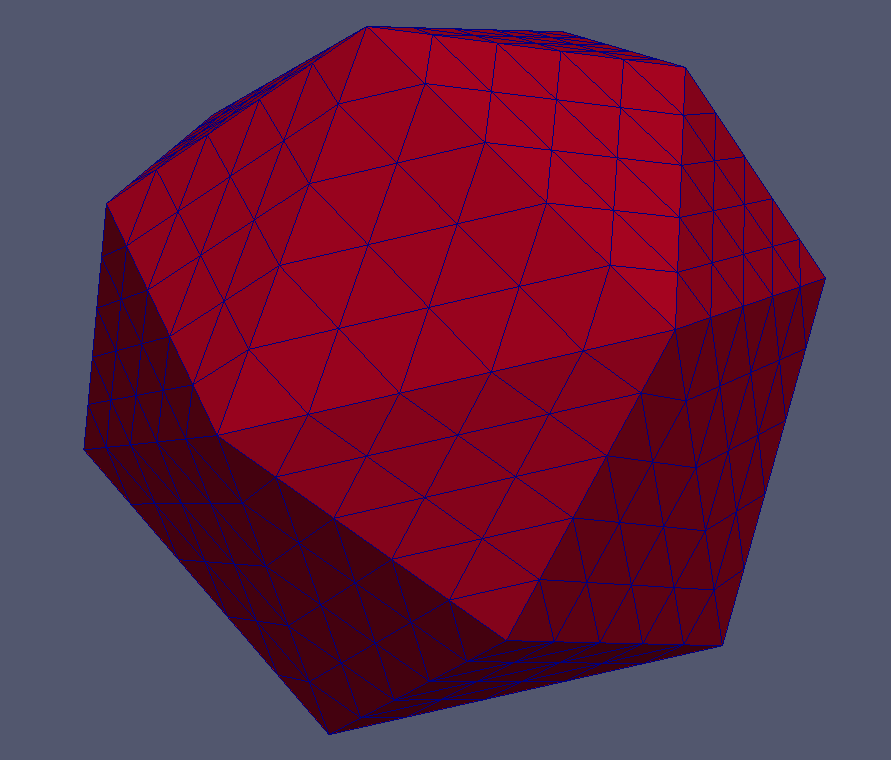
\includegraphics[scale=0.215]{images/sphere32discr6ord1} \end{subfigure}
	\begin{subfigure}[b]{0.48\textwidth} 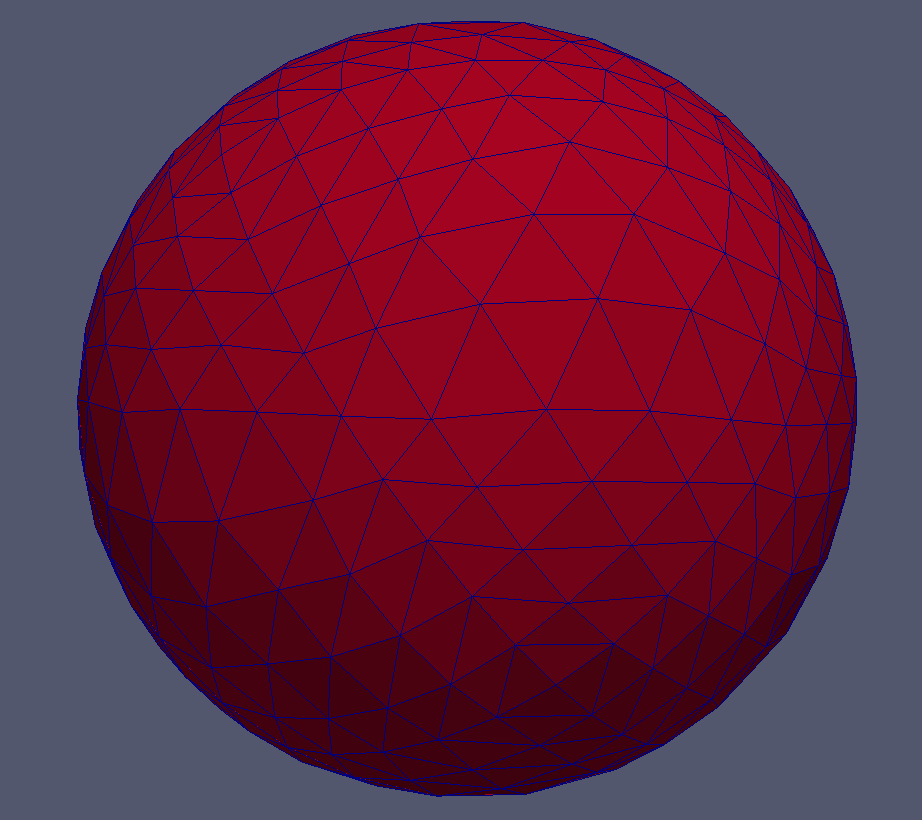
\includegraphics[scale=0.2]{images/sphere32discr6ord5} \end{subfigure}
	\captionsetup{width=0.8\textwidth} 
	\caption{Presented is the 32 element tetrahedral mesh of a sphere, using first and fifth order polynomial interpolation. Visualisation software (\ParaView{}, in this case) does not appear to have documented interface for direct curvilinear element output. The curvature is represented by virtual refinement of curvilinear tetrahedra into smaller linear tetrahedra }
	\label{fig:result:spherecurv}
\end{figure}

\noindent
Further, the accuracy of a PDE solution improves much faster with increasing basis function order (\textit{p}-refinement) than with increasing element number (\textit{h}-refinement) \cite{jin2014}, \cref{fig:jin:basisconv}. Fahs \cite{fahs2011} shows that, in case of curved material boundaries, this effect can only be exploited if the corresponding element geometries are of sufficiently high order \cref{fig:fahs:curvconv}.

\begin{figure}
    \centering
    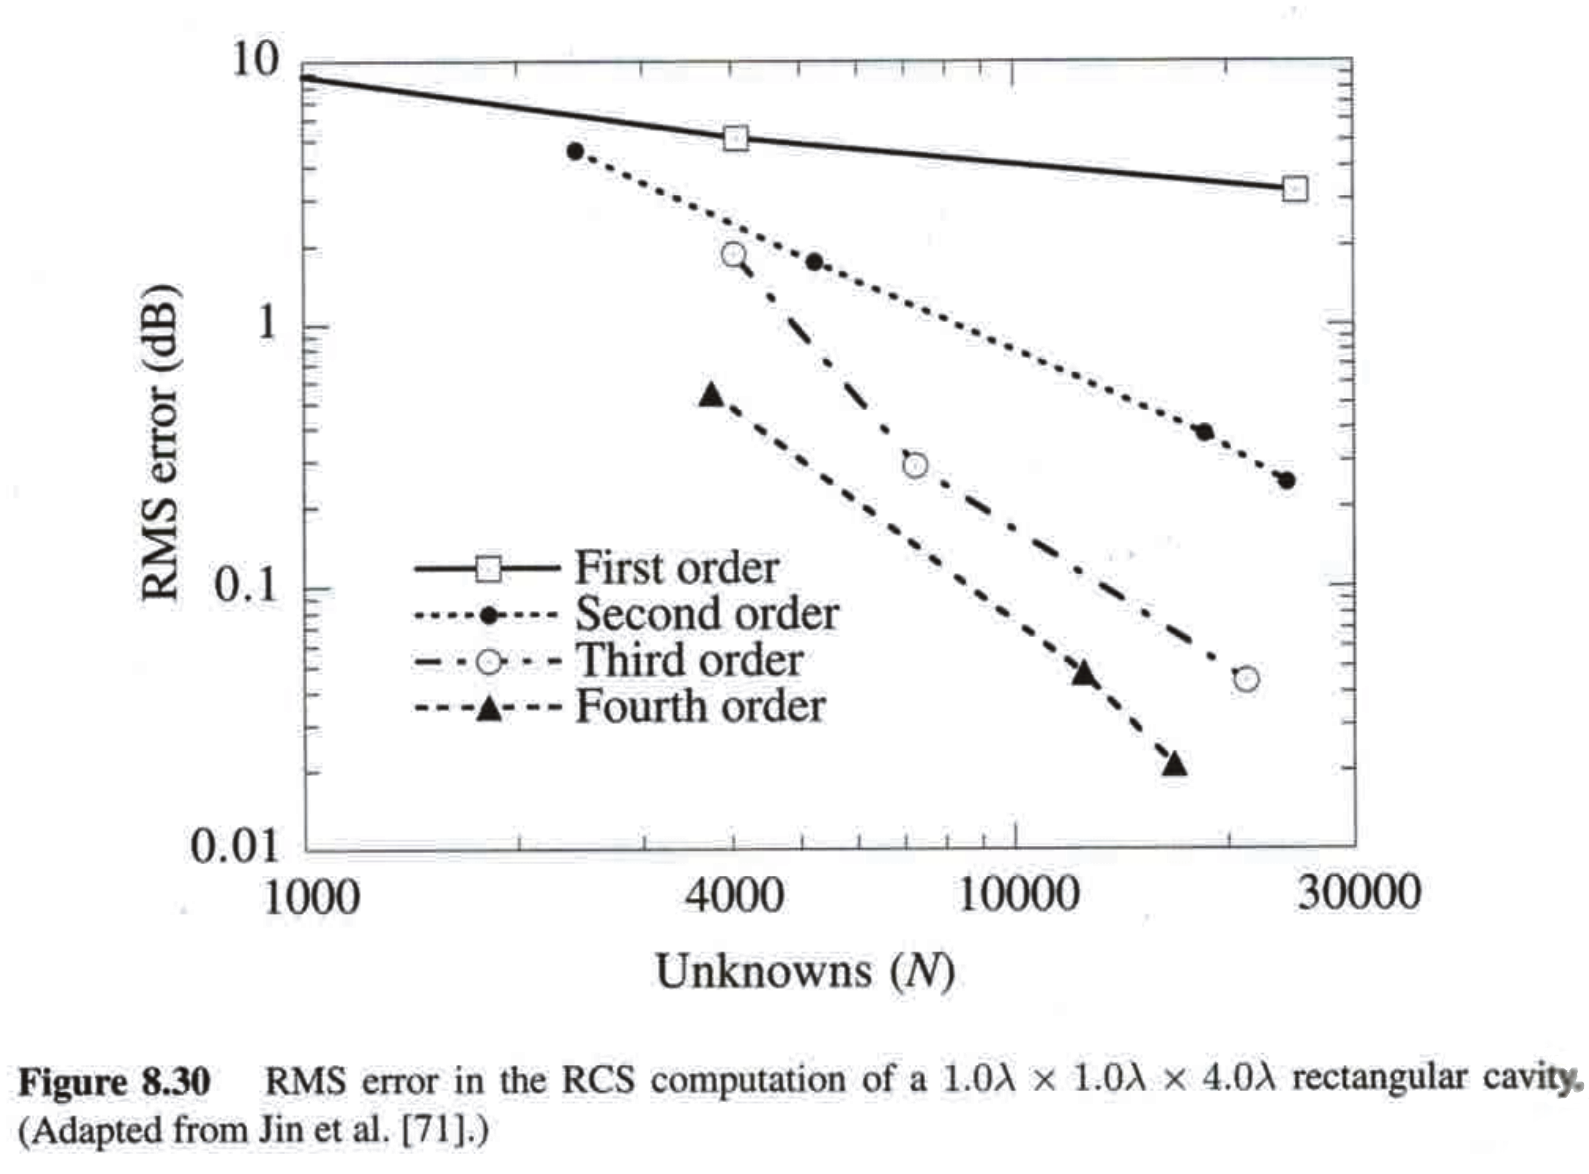
\includegraphics[scale=0.2]{images/jin-tfemim-3ed-fig8-30}
	\captionsetup{width=0.8\textwidth} 
	\caption{ Jin \cite{jin2014} shows that the improvement of accuracy due to h-refinement improves exponentially with increasing basis order. We thank the author for permission to reproduce this plot. }
	\label{fig:jin:basisconv}
\end{figure}

\begin{figure}
    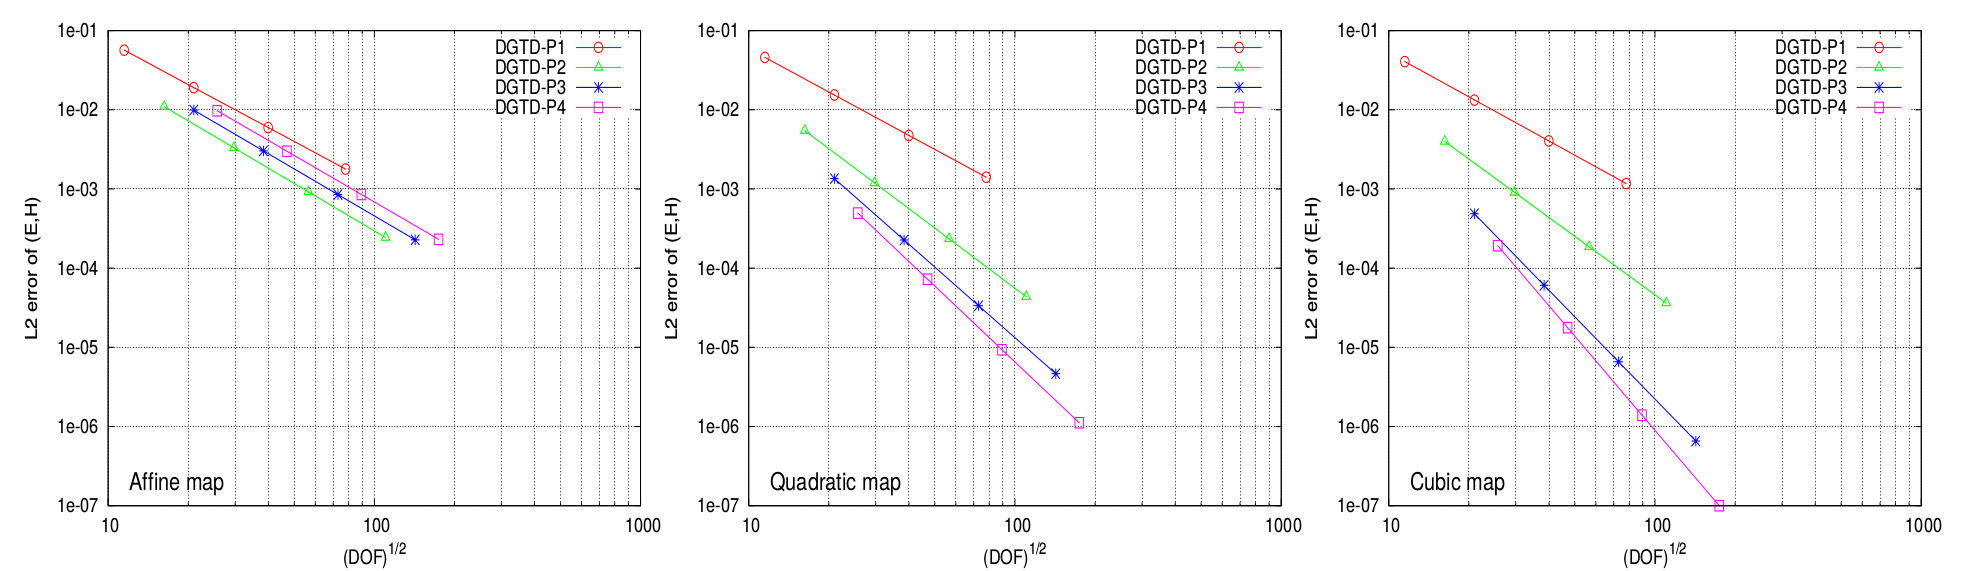
\includegraphics[scale=0.25]{images/fahs-convergence}
	\captionsetup{width=0.8\textwidth} 
	\caption{ Fahs \cite{fahs2011} shows that computational accuracy (in terms of $L_2$ norm) improves with increasing basis function order, but it improves faster if the entity interpolation (curvature) order is increased accordingly. We thank the author for permission to reproduce these plots.}
	\label{fig:fahs:curvconv}
\end{figure}


\subsection{Capabilities of CurvilinearGrid}
\label{section-outline-capabilities}

The \curvgrid{} is a self-consistent grid manager supporting 3D tetrahedral curvilinear grids. It depends on the core modules of \dune{} \citeDune{}, as well as an external parallel mesh partition library \ParMETIS \citeParMetis{}. \curvgrid{} also depends on \curvgeom{}, which we developed as a separate \dune{} module. \\

\noindent
\curvgeom{} is capable of interpolating and performing multiple geometric operations over curvilinear simplex entities (edges, triangles and tetrahedra) of orders 1-5 via hard-coded \textit{Lagrange} polynomials, and arbitrary order simplex entities via analytic \textit{Lagrange} interpolation method. \curvgeom{} complies with the standard \dunegeom{} interface, providing methods for local-to-global and global-to-local coordinate mapping, computation of the \textit{Jacobian} matrix, integration element and entity volume. \curvgeom{} has non-cached and cached implementations, where the cached version pre-computes the local-to-global map and its determinant, thus performing considerably faster for integration and mapping tasks. In comparison with the standard \dunegeom{}, \curvgeom{} provides methods to obtain either all interpolatory vertices of an entity or only its corners, as well as the method to obtain the curvilinear order. Additionally, \curvgeom{} provides the methods to obtain the outer normals of subentities of the geometry, and the subentity geometries themselves. Another feature of \curvgeom{} is the symbolic polynomial class and associated differential methods, which allow to obtain analytical expressions for local-to-global map and associated integration element, enabling exact manipulation of geometries of arbitrary order. \curvgeom{} contains its own recursive integration tool, wrapping the quadrature rules provided by dune-geometry. The reason for implementing this functionality is to accurately treat non-polynomial integrands for which the optimal polynomial order required for the desired accuracy is not known. In particular, it happens that curvilinear integration elements are non-polynomial in the general case (see \cref{sec:theory:integration}). The recursive integration scheme is capable to simultaneously integrate multidimensional integrands, such as vectors and matrices. This is highly useful, for example, for integrating outer product matrices. For such matrices the evaluation of all matrix elements at a given coordinate only requires $O(N)$ expensive function evaluations. \curvgeom{} provides a utility for testing curvilinear entities for self-intersection. This is done by sampling the value of integration element across the entity, and ensuring that it never changes sign. \\

\begin{figure}[H]
    \centering
    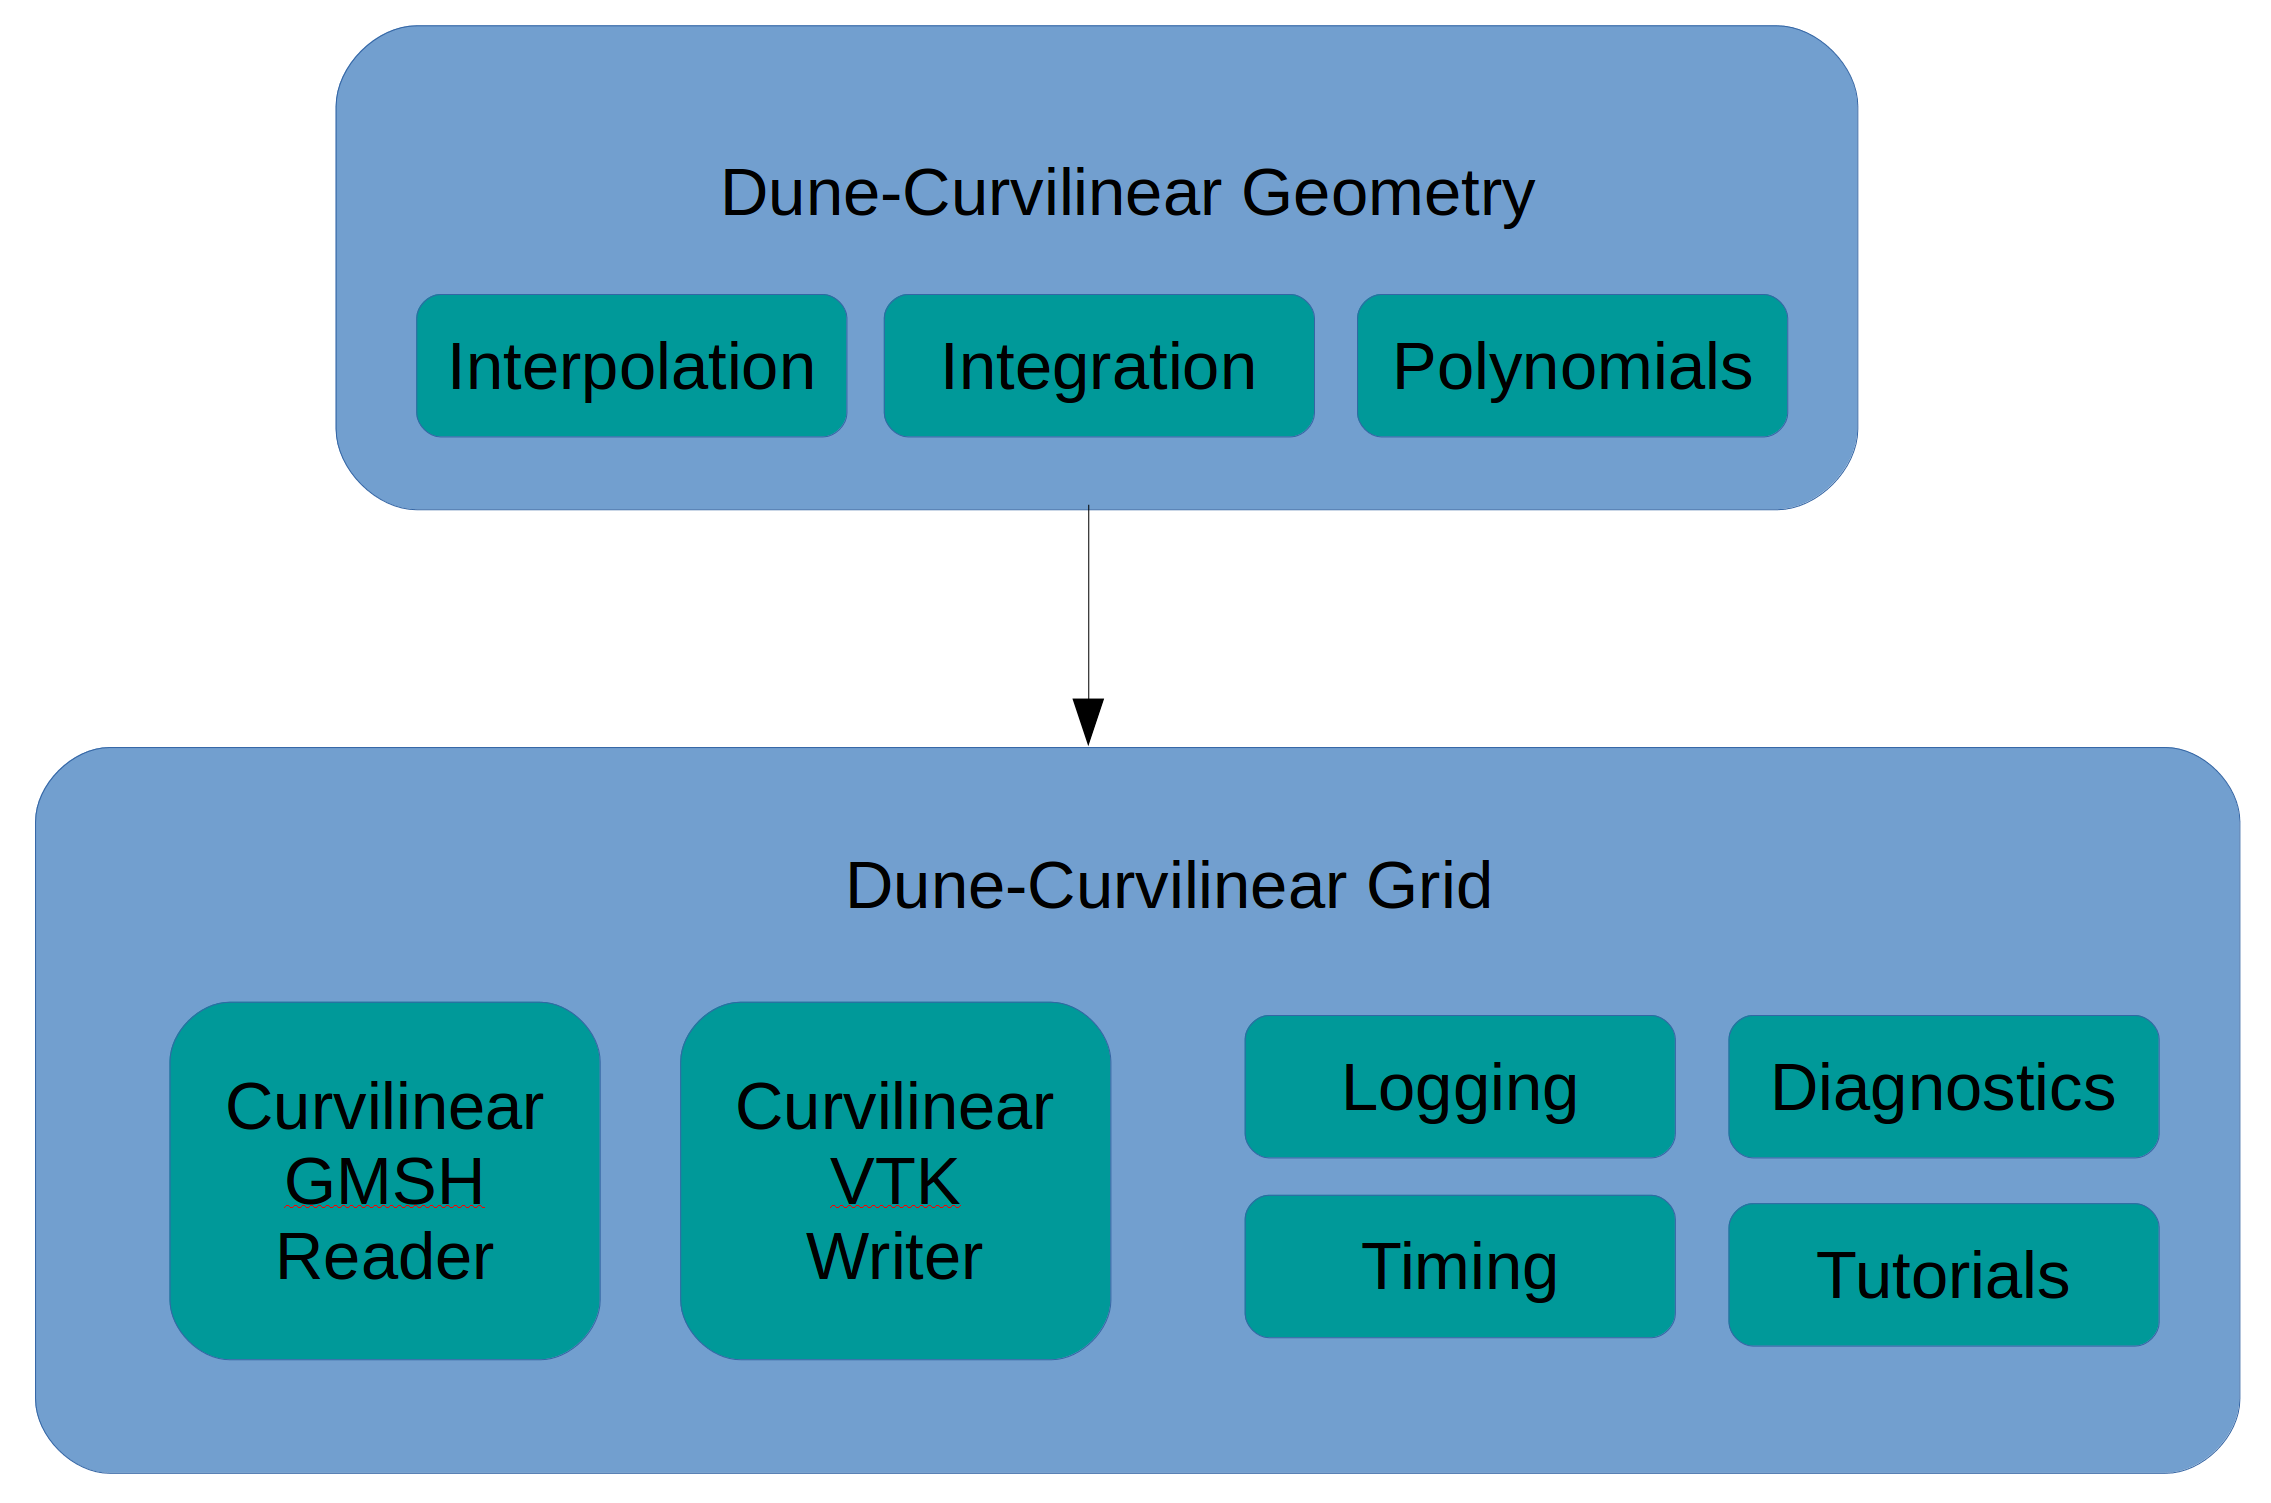
\includegraphics[scale=0.15]{images/curvgrid-map}
    \caption{The strucure of \curvgrid{}}
    \label{fig:introduction:curvgrid:structure}
\end{figure}

\noindent
\curvgrid{} module manages the entire process of reading, manipulating, and writing of curvilinear geometries and associated fields (e.g. PDE solution). The former is accomplished by \textit{Curvilinear GMSH Reader} (\curvreader{}) class. \curvreader{} is currently capable of reading curvilinear \textit{.msh} files of orders 1 to 5, where 1 corresponds to linear meshes. \curvreader{} is fully parallel and scalable for large parallel architectures. Each process only reads the necessary local part of the mesh, distributing the memory equally among all processes. It must be noted that earlier implementation of \textit{GMSH Reader} in the \dunegrid{} module suffered from serial reading of the mesh on the master process, which is no longer a bottleneck in our implementation. \curvreader{} has the option to partition the mesh using \ParMETIS{} during the reading procedure before reading the curvature vertices, further decreasing the file access time. \curvreader{} also reads material elementary and boundary tags provided by \gmsh{}. It extends the standard \textit{Grid Factory} interface, providing tag information, as well as curvilinear order. The grid output is accomplished by \textit{Curvilinear VTK Writer} (\curvwriter{}) module, supporting \textit{VTK}, \textit{VTU} and \textit{PVTU} file formats. \curvwriter{} can either write the entire grid automatically, or write a set of individual entities, one at a time. When writing the entire grid, each element is supplied by fields denoting its rank, partition type (\cref{fig:result:spherestruct}) and physical tag, which can be used to visually inspect the parallel connectivity of the domain. The scalability of the grid assembly and visualisation has been tested on parallel architectures containing from 12 to 128 cores. By the time of writing, the \curvgrid has been successfully run on several dozen different meshes, the largest being the 4.4 million element tetrahedral mesh \cref{fig:result:bullseye}. The user has full flexibility to define the codimensions of the entities that will be written, the choice to write interior, domain, process boundaries and/or ghost elements, as well as the order of virtual refinement of curvilinear entities. The output mesh can be supplied with an arbitrary number of vector and scalar fields representing, for example, the solution(s) of a PDE. We have tested the visualisation capabilities of \curvgrid{} using \ParaView{} \cite{johnson+2005} and \visit{} \cite{childs+2012} end user software. \\

\begin{figure}[H]
	\begin{subfigure}[b]{0.30\textwidth} \hspace{4mm} 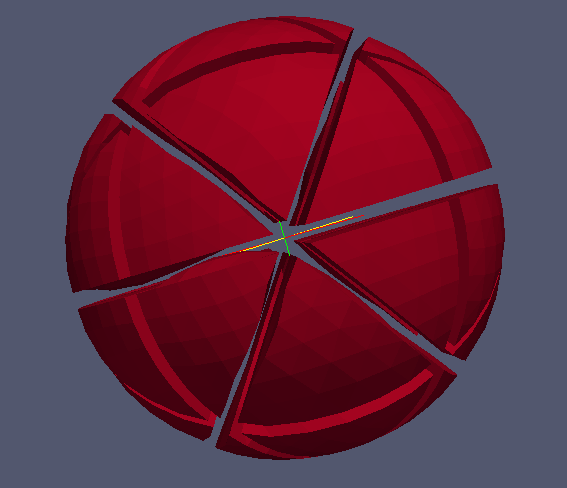
\includegraphics[scale=0.22]{images/32-inter} \captionsetup{width=0.8\textwidth} \caption{ Interior elements } \end{subfigure}
	\begin{subfigure}[b]{0.30\textwidth} \hspace{4mm} 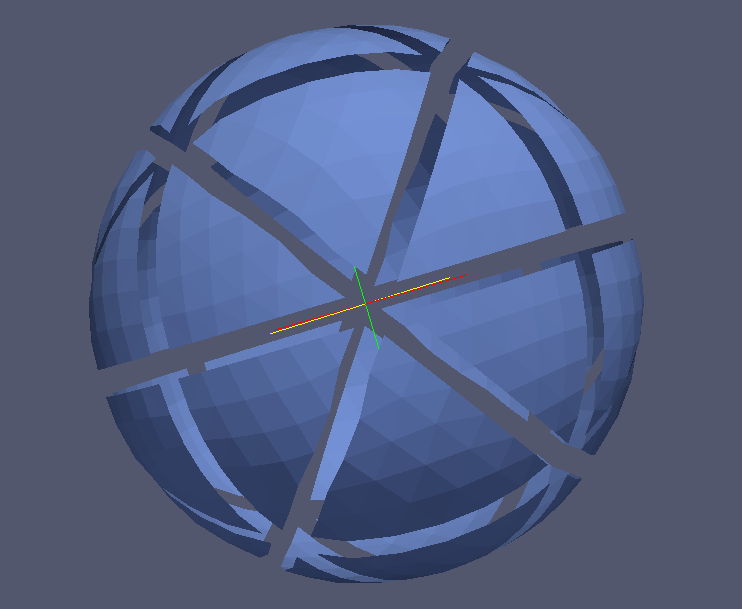
\includegraphics[scale=0.18]{images/32-db}    \captionsetup{width=0.8\textwidth} \caption{ Domain Boundary surfaces} \end{subfigure}
	\begin{subfigure}[b]{0.33\textwidth} \hspace{4mm} 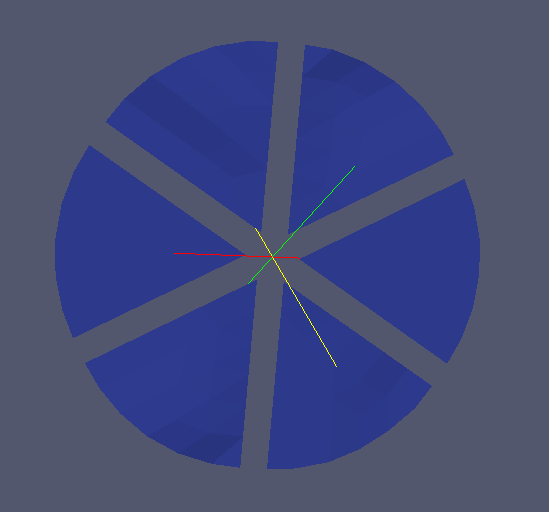
\includegraphics[scale=0.22]{images/32-pb}    \captionsetup{width=0.8\textwidth} \caption{ Interprocessor Boundary surfaces} \end{subfigure}
	\begin{subfigure}[b]{0.46\textwidth} \vspace{5mm} \hspace{12mm} 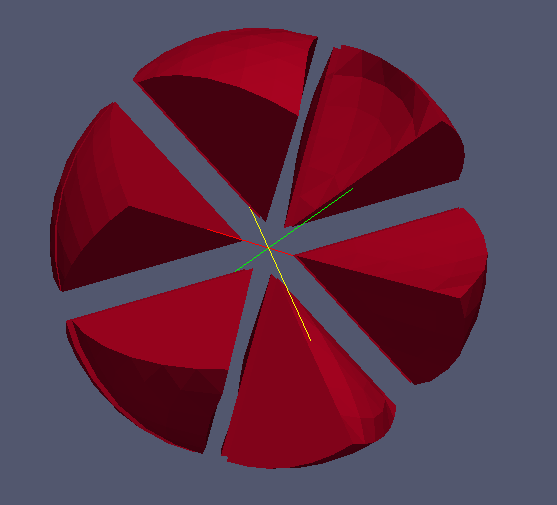
\includegraphics[scale=0.25]{images/32-ghost} \captionsetup{width=0.6\textwidth} \caption{ Ghost elements, borrowed from neighboring processes} \end{subfigure}
	\begin{subfigure}[b]{0.46\textwidth} \vspace{5mm} \hspace{12mm} 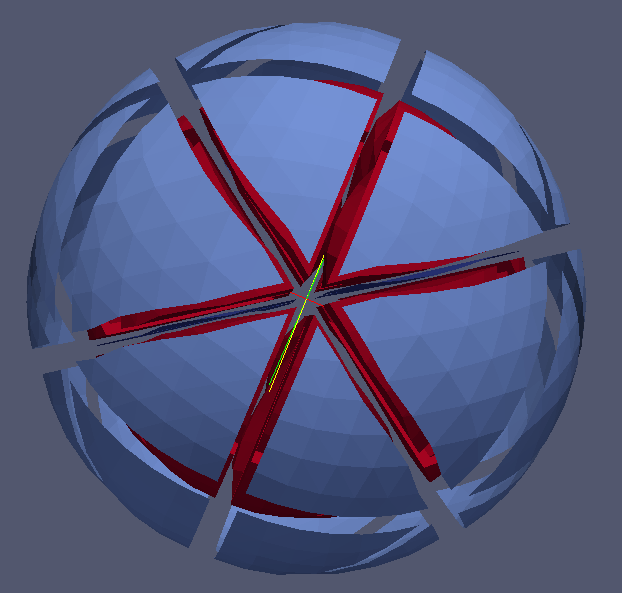
\includegraphics[scale=0.21]{images/32-full}  \captionsetup{width=0.6\textwidth} \caption{ Entities of all structural types visualised at the same time } \end{subfigure}
	\caption{ Visualisation of various structural (partition) types of a 32 element tetrahedral mesh, loaded in parallel on 2 cores }
	\label{fig:result:spherestruct}
\end{figure}

\begin{figure}[H]
    \centering
	\begin{subfigure}[b]{0.48\textwidth} 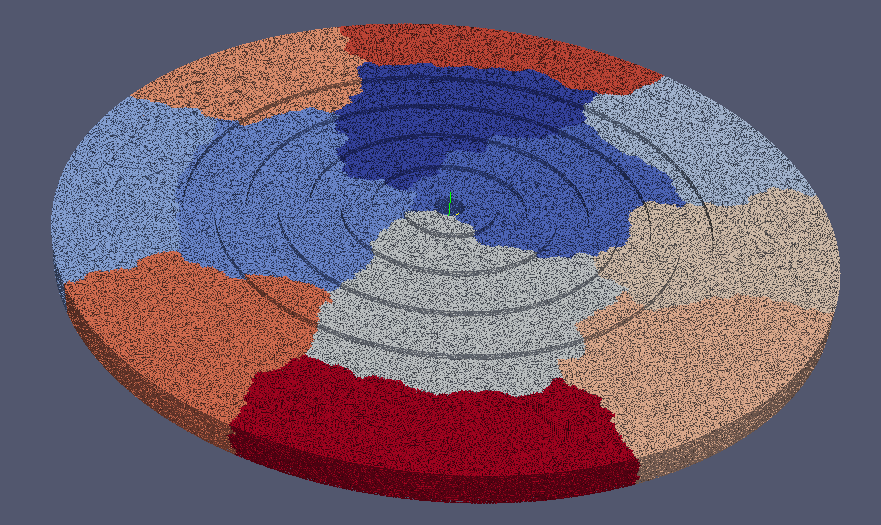
\includegraphics[scale=0.20]{images/bullseye-core-angle}          \captionsetup{width=0.8\textwidth} \caption{Interior elements coloured by owner process rank}   \end{subfigure}
	\begin{subfigure}[b]{0.48\textwidth} 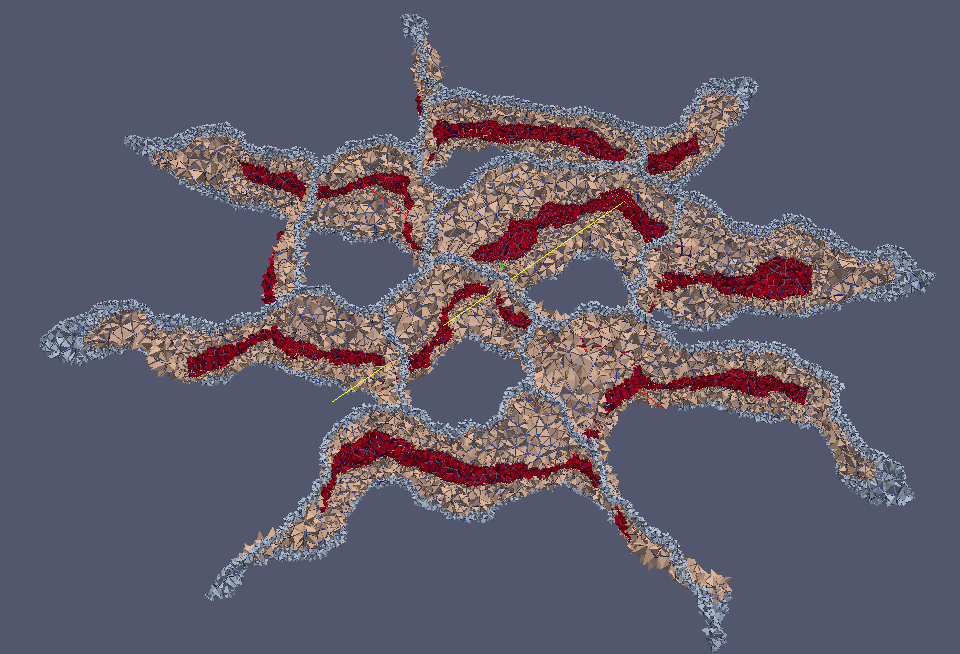
\includegraphics[scale=0.17]{images/bullseye-ghostelements-angle}  \captionsetup{width=0.8\textwidth} \caption{Ghost elements, coloured by material tag} \end{subfigure}
	\caption{Interior and ghost elements of a 4.4 million element tetrahedral mesh of the Bullseye geometry}
	\label{fig:result:bullseye}
\end{figure}

\noindent
The core of \curvgrid{} provides the essential indexing and communication capabilities. The global and local indices are provided for entities of all codimensions. Interprocessor communication is performed via the \dune{} standard \textit{DataHandle} interface for provided \textit{Ghost} elements entities of all codimensions. As an extension to the \dunegrid{} interface, it is possible to directly address the core curvilinear geometry of each entity, as well as the associated physical tags. \curvgrid{} is also equipped with a set of useful utilities:
\begin{itemize}
    \item \textit{Timing mechanisms}: parallel timing of separate parts of the code with statistics output over all processes
    \item \textit{Logging mechanisms}: real time logging of the current state of the code, as well as the current memory consumption on each core of a machine, allowing for the real-time diagnostics of memory bottlenecks of the code.
    \item \textit{Nearest-neighbour communication} - wrapper for the implementation of \textit{MPI\_Neighbor\_alltoall} for vector communication with neighboring processes. This functionality is available as of the MPI-2 standard \cite{MPI-3.1}
    \item \textit{Global boundary container} - interior/domain boundary all-to-all communication, useful for dense PDE solvers, such as the Boundary Integral method. \cite{kern+2009}
    \item \textit{Grid diagnostics} - collects statistics on entity volumes, qualities and their distribution among processes
\end{itemize}

%%%\subsection{Design decisions}
%%%\label{section-outline-designdecisions}
%%%
%%% Design decisions for Curvilinear Grid Factory
%%%\begin{itemize}
%%%	\item User must provide globalId's for vertices and elements. [Automatically implemented by \gmsh{} \citeGMSH]
%%%	\item User must provide all boundary segments inside \gmsh{} file.
%%%\end{itemize}


% \subsection{Internal Structure}
% \label{section-outline-internalstructure}
% 
% Below we present a simplified structure of classes used by Curvilinear Grid and geometry \\

% \noindent
% \begin{tabularx}{\textwidth}{ l | X }
% \hline
%    Class Name & Description \\ \hline
%    CurvilinearGeometry                & Core class complying with dune-geometry standard \\ \hline
%    * CurvilinearGeometryHelper        & Auxiliary functions, subentities for curvilinear elements \\ \hline
%    * LagrangeInterpolator             & \textit{Lagrange} Interpolation of element geometry \\ \hline
%    * Polynomial                       & Analytic polynomial routines \\ \hline
%    * DifferentialHelper               & Analytic Curvilinear Jacobians and Integration elements \\ \hline
%    * IntegralHelper                   & Integral Functors, analytic integration routines  \\ \hline
%    * QuadratureIntegrator             & Recursive integration using numerical quadrature. Performs fast \\ \hline
%    * AdaptiveIntegrator               & Recursive integration using adaptive refinement. Performs slowly \\ \hline
%   CurvilinearGMSHReader               & Reads a $.msh$ file and supplies entities to a Grid Factory \\ \hline
%   * Gmsh2DuneMapper                   & Converts between interpolation vertex numbering paradigms \\ \hline
%   CurvilinearVTKWriter                & Writes curvilinear elements to VTK, VTU/PVTU files \\ \hline
%   CurvilinearVTKGridWriter            & Writes Curvilinear Grid to VTK, VTU/PVTU files \\ \hline
%   CurvilinearGridBase                 & Lower level grid implementation. All entities are given by their codimension and index \\ \hline
%   * CurvilinearGridStorage            & Storage class for entire grid \\ \hline
%   * CurvilinearGridConstructor        & Constructs entities of the grid, finds neighbouring processes, generates global index \\ \hline
%   * CurvilinearGhostConstructor       & Constructs ghost entities \\ \hline
%   * CurvilinearPostConstructor        & Enables DataHandle communication \\ \hline
%   Curvilinear Grid                    & Core class complying with dune-grid standard \\ \hline
%   * CurvilinearGridFactory            & Interface for constructing Curvilinear Grid \\ \hline
%   * CurvilinearGridDiagnostics        & Tests and collects statistics on Curvilinear Grid \\ \hline
%   * LoggingMessage                    & Logging output with varying levels of verbosity \\ \hline
%   * LoggingTimer                      & Parallel timing of parts of code. \\ \hline
%   * AllCommunicate                    & Nearest neighbour communication for POD. Wrapper for $MPI\_alltoallv$ \\ \hline
%   * VectorHelper                      & Manipulation of vectors (union, intersection, complement), as well as conversion to string \\ \hline
% \end{tabularx}
